% Monitoramento de servidores Linux por web sites.
%====================================================================================================
% TCC
%----------------------------------------------------------------------------------------------------
% Autor				    : Eduardo Balan
% Orientador		  : Kleber Krugrer
% Instituição 		: UFMS - Universidade Federal do Mato Grosso do Sul
% Departamento		: CPCX - Sistema de Informação
%----------------------------------------------------------------------------------------------------
% Data de criação	: 29 de Março de 2017
%====================================================================================================

\chapter{Fundamentação Teórica}\label{cap:funTeorica}

Neste Capítulo são apresentados os conceitos utilizados neste trabalho de acordo com a literatura estudada. Na seção \ref{sec:ArquiteturaClienteServidor} explica-se os conceitos da arquitetura cliente-servidor. Na Seção \ref{sec:WebServices} explicase os conceitos de um \textit{web-service}. Na Seção \ref{sec:BancodeDados} explica-se o conceito de Banco de Dados. Na Seção \ref{sec:Http} explica-se o conceito do protocolo HTTP/1.1 seus metodos forma de utilização e respostas esperadas. Na Seção \ref{sec:ArquiteturaReST} é apresentada o estilo de desenvolvimento da arquitetura ReST e na Seção \ref{sec:TestesAutomatizados} são mostradas as principais vantagens e melhorias adquiridas por meio dos testes automatizados.


\section{Arquitetura Cliente-Servidor}\label{sec:ArquiteturaClienteServidor}

		Em uma arquitetura cliente-servidor há um hospedeiro sempre em funcionamento, denominado servidor, que atende à requisições de muitos outros hospedeiros, denominados clientes. Estes podem estar em funcionamento esporadicamente ou a todo o tempo. Um exemplo clássico é a aplicação \textit{web} na qual um servidor \textit{web} que está sempre em funcionamento atende à requisições de \textit{browsers} de hospedeiros clientes. Ao receber uma requisição de um objeto de um hospedeiro cliente, o servidor \textit{web} responde enviando o objeto requisitado a ele. Observe que, na arquitetura cliente-servidor, os clientes não se comunicam diretamente uns com os outros: por exemplo, na aplicação \textit{web}, dois \textit{browsers} não se comunicam diretamente. Outra característica da arquitetura cliente-servidor é que o servidor tem um endereço fixo, bem conhecido, denominado endereço IP (\textit{Internet Protocol}). Devido a esse característica do servidor e devido ao fato de ele estar sempre em funcionamento, um cliente sempre pode contatá-lo enviando um pacote ao endereço do servidor. Algumas das aplicações mais conhecidas que empregam a arquitetura cliente-servidor são \textit{web}, FTP (\textit{File Transfer Protocol}), Telnet e e-mail. Essa arquitetura cliente-servidor é mostrada na \autoref{Img:ArquiteturaClienteServidor} em que diversos clientes utilizando, computadores, notebooks e celulares realizam comunicação com um servidor \cite{Kurose:2010}.

Em aplicações cliente-servidor, muitas vezes acontece de um único hospedeiro servidor ser incapaz de atender a todas as requisições de seus clientes. Um site \textit{web} pode ficar rapidamente saturado se tiver apenas um servidor para atender grande número de requisições. Por essa razão, um grande conjunto de hospedeiros - às vezes coletivamente chamados \textit{data center} - freqüentemente é usado para criar um servidor virtual poderoso em arquitetura cliente-servidor, aumentando a capacidade de resposta de requisições \cite{Kurose:2010}.


\begin{figure}
	\centering
	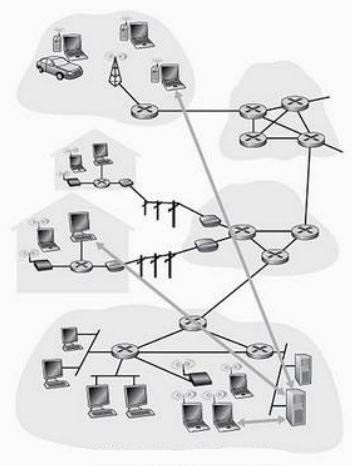
\includegraphics[width=0.5\textwidth]{figuras/KuroseClienteServidorpg88.jpg}
	\caption[Arquitetura Cliente-Servidor.]{Representa a arquitetura clitente-Servidor, onde diversos tipos de cliente se comunicam com um mesmo servidor.}
	\label{Img:ArquiteturaClienteServidor}
\end{figure}


\section{\textit{Web Services}}\label{sec:WebServices}


O \textit{Web Service} é um \textit{software}  que atende a uma função de negócio específica para seus clientes. Ele recebe requisições de clientes e as responde ocultando todo o detalhamento do seu processamento. Normalmente as transações estão em formato XML (\textit{Extended Markup Language}), e são transmitidas utilizando o protocolo HTTP (HyperText Transfer Protocol), entretanto podem ser utilizados outros protocolos de transporte \cite{Sampaio:2003}.

Os \textit{Web Services}, aliados aos padrões estabelecidos da Internet, podem fazer com que os dados fluam entre as várias entidades, como o governo e empresas interagindo entre si, reduzindo custos de modo a possibilitar maior facilidade e rapidez na troca de informações \cite{Abinader:2006}. Um exemplo utilizado nacionalmente é a NF-e (Nota Fiscal Eletrônica) em que diversas empresas com \textit{softwares} diferentes enviam arquivos xml utilizando o protocolo https (\textit{Hyper Text Transfer Protocol Secure}) para o \textit{web service} da receita federal, aguardam a realização dos processamentos de validação e recebem um arquivo xml de retorno com as informações desejadas.

Um \textit{web wervice} deve executar unidades completas de trabalho, não dependendo do estado de outros componentes externos. Outra definição importante é que eles devem ser "\textit{Stateless}" ou seja, cada requisição é considerada uma transação independente que não está relacionada a qualquer requisição anterior de forma que a comunicação consista de pares de requisição e resposta independentes \cite{Sampaio:2003, W3C:2001}.


\section{Banco de Dados} \label{sec:BancodeDados}

Um Sistema de banco de dados é basicamente um sistema computadorizado de manutenção de registros. O banco de dados, por si só, pode ser considerado como o equivalente eletrônico de um armário de arquivamento; ou seja, ele é um repositório ou recipiente para uma coleção de arquivos de dados computadorizados. Os usuários de um banco de dados podem solicitar que o sistema realize diversas operações envolvendo tais arquivos, por exemplo:
\begin{itemize}
		\item Acrescentar novos arquivos ao banco de dados
		\item Inserir dados em arquivos existentes 
		\item Buscar dados de arquivos existentes
		\item Excluir dados de arquivos existentes
		\item Alterar dados em arquivos existentes
		\item Remover arquivos existentes do Banco de dados
\end{itemize}

As informações contidas no banco de dados em questão podem ser qualquer coisa que tenha algum significado ou indivíduo ou à organização a que o sistema deve servir, ou seja, qualquer coisa que seja necessária para auxiliar no processo geral das atividades desse indivíduo ou dessa organização

Os sistemas de bancos de dados Estão disponíveis em máquinas que variam desde pequenos computadores de mão (hand-helds e celulares) ou computadores pessoais até os maiores mainframes ou clusters de computadores de grande porte. Normalmente sistemas em máquinas grandes costumam ser multiusuários, enquanto os que estão em máquinas menores tendem a ser de monousuários. Um sistema monousuário é um sistema em que no máximo um usuário pode acessar o banco de dados em determinado momento; um sistema multiusuário é aquele em que muitos usuários podem acessar o banco de dados ao mesmo tempo; porém, a distinção é irrelevante para a maioria dos usuários, pois um dos objetivos dos sistemas multiusuários, em geral, é que cada usuário se comporte como se estivesse trabalhando com um sistema monousuário.


As informações contidas no banco de dados são persistentes, ou seja, uma vez que um operação de inserir é aceita pelo SGBD (Sistema de Gerenciamento de Banco de Dados), ela só poderá ser removida por outra requisição explicita ao SGBD, e não como um mero efeito colateral, como algum programa concluindo sua execução apagar todos os registros.


As transações realizadas pelo SGBD utilizam o conceito de ACID(Atomicidade, Consistência, Isolamento e Durabilidade):

\begin{itemize}
		\item Atomicidade quer dizer que um bloco de transações deve ter todas as suas operações executadas em caso de sucesso ou nenhum operação executada, mesmo que o sistema venha a falha.
		\item Consistência diz que a execução de uma transação deve levar o banco de dados de um estado consistente a um outro estado consistente, dessa forma, uma transação deve respeitar as regras de integridade dos dados
		\item Isolamento quer dizer que transações paralelas não interferem umas nas outras, ou seja, se um usuário tentar alterar o salario de um funcionário e outro usuário tentar alterar o mesmo salario ao mesmo tempo uma transação só iniciara quando a outra for completamente terminada.
		\item Durabilidade diz que as transações com sucesso devem persistir no banco de dados mesmo em caso de falha.
\end{itemize}



\section{HTTP/1.1 \textit{HyperText Transfer Protocol}} \label{sec:Http}

O protocolo HTTP (\textit{HyperText Transfer Protocol}) é o protocolo utilizado em toda a \textit{World Wide Web}. Ele especifica o formato das mensagens que os clientes enviam aos servidores e também o formato de respostas que receberão. Cada interação consiste em uma solicitação ASCII, seguida por uma resposta RFC 822. 

Na utilização do protocolo HTTP/1.1 todos os clientes e todos os servidores devem obedecer a esse protocolo que é definido na RFC 2616 \cite{Tanenbaum:2003}.

\subsection{Conexões} \label{HTTP/1.1 - HyperText Transfer Protocol}

O modo habitual de cliente entrar em contato com um servidor é estabelecer uma conexão TCP (\textit{Transmission Control Protocol}) para a porta 80 da máquina servidora, embora esse procedimento não seja exigido formalmente. A vantagem de se usar o TCP é que ambas as partes não têm de se preocupar com mensagens perdidas, mensagens duplicadas, mensagens longas ou confirmações. Todos esses assuntos são tratados pela implementação do TCP \cite{Tanenbaum:2003}.

O HTTP/1.1 diferentemente de seus antecessores, admite conexões persistentes. Com elas, é possível estabelecer uma conexão TCP, enviar uma solicitação e obter uma resposta, e depois enviar solicitações adicionais e receber respostas adicionais. Amortizando o custo da instalação e
da liberação do TCP por várias solicitações, o processamento relativo devido ao TCP é muito menor por solicitação. Também é possível transportar as solicitações por \textit{pipeline}, ou seja, enviar a segunda solicitação antes de chegar a resposta da primeira \cite{Tanenbaum:2003}.



\subsection{Métodos} \label{subsec:Metodos}

O HTTP foi criado de modo mais geral que simplesmente para utilização na \textit{web}, visando às futuras aplicações orientadas a objetos. Por essa razão, são aceitas operações chamadas métodos, diferentes da simples solicitação de uma página da \textit{web}. Cada solicitação consiste em uma ou mais linhas de texto ASCII, sendo a primeira palavra da primeira linha o nome do método solicitado. Os métodos internos estão listados na \autoref{Tab:MetodosHTTP} \cite{Tanenbaum:2003}.


% Please add the following required packages to your document preamble:
% \usepackage[table,xcdraw]{xcolor}
% If you use beamer only pass "xcolor=table" option, i.e. \documentclass[xcolor=table]{beamer}
\begin{table}[!ht]
\centering
\begin{tabular}{|l|l|}
\hline
{\color[HTML]{000000} \textbf{Método}} & {\color[HTML]{000000} \textbf{Descrição}} 
\\ \hline
GET                                    & \multicolumn{1}{p{13.50cm}|}{O método GET solicita ao servidor que envie a página (ou objeto, no caso mais genérico; na prática,apenas um arquivo). A grande maioria das solicitações a servidores da \textit{web} tem a forma de métodos GET.} 
\\ \hline
HEAD                                   & \multicolumn{1}{p{13.50cm}|}{O método HEAD solicita apenas o cabeçalho da mensagem, sem a página propriamente dita. Essemétodo pode ser usado para se obter a data da última modificação feita na ágina, para reunirinformações destinadas à indexação, ou apenas para testar a validade de um URL(Uniform Resource Locator).}
\\ \hline
PUT                                    & \multicolumn{1}{p{13.50cm}|}{O método PUT grava em uma página já existe. Esse método possibilita a criação de um conjunto de páginas da \textit{web} em um servidor remoto. O corpo da solicitação contém a página. } 
\\ \hline
POST                                   & \multicolumn{1}{p{13.50cm}|}{O método POST grava novos dados e são "anexados" a ele, em um sentido mais genérico\cite{Tanenbaum:2003}.} 
\\ \hline
DELETE                                 & \multicolumn{1}{p{13.50cm}|}{O método DELETE exclui a página. Não há garantia de que DELETE tenha sido bem-sucedido pois, mesmo que oservidor HTTP remoto esteja pronto para excluir a página, o arquivo subjacente pode ter um modoque impeça o servidor HTTP de modificá-lo ou excluí-lo \cite{Tanenbaum:2003}. }
\\ \hline
TRACE                                  & \multicolumn{1}{p{13.50cm}|}{O método TRACE serve para depuração. ele instrui o servidor a enviar de volta a solicitação. Essemétodo é útil quando as solicitações não estão sendo processadas corretamente e o cliente desejasaber qual solicitação o servidor recebeu de fato \cite{Tanenbaum:2003}.}   
\\ \hline
CONNECT                                & \multicolumn{1}{p{13.50cm}|}{O método CONNECT não é usado atualmente. Ele é reservado para uso futuro \cite{Tanenbaum:2003}.} \\ \hline
OPTIONS                                & \multicolumn{1}{p{13.50cm}|}{O método OPTIONS fornece um meio para que o cliente consulte o servidor sobre suas propriedades ou sobre as de um arquivo específico \cite{Tanenbaum:2003}.}
\\ \hline
\end{tabular}
\caption[Métodos da solicitações HTTP.]{Métodos da solicitações HTTP e suas descrições \cite{Tanenbaum:2003}.}
\label{Tab:MetodosHTTP}
\end{table}





\subsection{Códigos de Resposta} \label{subsec:Resposta}

Toda solicitação obtém uma resposta que consiste em uma linha de status e, possivelmente,
informações adicionais (por exemplo, uma página da \textit{web} ou parte dela). A linha de status contém
um código de status de três dígitos informando se a solicitação foi atendida e, se não foi, o motivo. 
O primeiro dígito é usado para dividir as respostas em cinco grupos importantes, como mostra-se na \autoref{Tab:FalhasHTTP} \cite{Tanenbaum:2003}.


% Please add the following required packages to your document preamble:
% \usepackage[table,xcdraw]{xcolor}
% If you use beamer only pass "xcolor=table" option, i.e. \documentclass[xcolor=table]{beamer}
\begin{table}[!h]
\centering
%\caption{My caption}
\begin{tabular}{|l|l|}
\hline
%\multicolumn{1}{|c|}{{\color[HTML]{000000} \textbf{Código}}} & \multicolumn{1}{c|}{{\color[HTML]{000000} \textbf{Descrição}}}    \\ \hline
\textbf{Código}   & \textbf{Descrição}       																						 \\ \hline
1xx   & Raramente são usados na prática \cite{Tanenbaum:2003}.        																						 \\ \hline
2xx   & Solicitação foi tratada com sucesso \cite{Tanenbaum:2003}.            																		 \\ \hline
3xx   & \begin{tabular}[c]{@{}l@{}}Informam ao cliente que ele deve procurar em outro lugar, 
				\\ usando uma URL diferente \cite{Tanenbaum:2003}.\end{tabular} 																						\\ \hline
4xx   & \begin{tabular}[c]{@{}l@{}}Solicitação falhou devido a um erro do cliente,
				\\ como uma solicitação inválida ou uma página inexistente \cite{Tanenbaum:2003}.\end{tabular}             \\ \hline
5xx   & \begin{tabular}[c]{@{}l@{}}O próprio servidor tem um problema, seja causado por um  
				\\ erro em seu código ou por uma sobrecarga temporária \cite{Tanenbaum:2003}.\end{tabular}                  \\ \hline
\end{tabular}
\caption[Códigos de resposta da solicitação HTTP.]{Códigos de resposta da solicitação HTTP \cite{Tanenbaum:2003}.}
\label{Tab:FalhasHTTP}
\end{table}


\subsection{Exemplo de utilização do HTTP/1.1} \label{subsec:ExemploHttp}

Este protocolo foi desenvolvido de maneira a ser o mais flexível possível para comportar diversas necessidades diferentes.
Sempre que uma requisição é enviada ela segue o formato da requisições que pode ser visto no \autoref{Func:GETModelo} \cite{Saudate:2014}.

\begin{lstlisting}[label=Func:GETModelo,caption={[Formato de uma requisição HTTP]Formato de uma requisição HTTP}]
<método> <URL> HTTP/<versão>
<Cabeçalhos - Vários cabeçalhos podem ser enviados mas um em cada linha>

<corpo da requisição> 
\end{lstlisting}


Quando um GET para http://www.site.com.br/clientes é realizado uma requisição é criada como pode ser visto no \autoref{Func:GETExemplo}. Nesta requisição pode ser visto em sua primeira linha o método GET da solicitação seguido pela URL a qual esta sendo feito a solicitação e pela versão do protocolo HTTP. O servidor responsável por receber a solicitação e a porta são passado no cabeçalho da requisição precedido por "Host:". Na terceira linha pode ser visto um cabeçalho \textit{Accept}, que serve para informar ao servidor qual tipo de dados a requisição espera receber \cite{Saudate:2014}.


\begin{lstlisting}[label=Func:GETExemplo,caption={[Exemplo de uma requisição HTTP utilizando o método GET.]Exemplo de uma solicitação HTTP utilizando o método GET, para http://www.site.com.br/clientes com o pedido de uma arquivo XML de resposta.}]
GET /clientes HTTP/1.1
Host: www.site.com.br:80
Accept: text/xml
\end{lstlisting}

Assim que o servidor receber a solicitação ele ira processar as informações, e retornara uma resposta com um dos código mostrado no \autoref{Tab:FalhasHTTP}. A resposta retornada possuirá o formato mostrado no \autoref{Func:RespostaModelo} \cite{Saudate:2014}.


\begin{lstlisting}[label=Func:RespostaModelo,caption={[Formato de uma resposta HTTP]Formato de uma resposta HTTP}]
HTTP/<versão> <código de status> <descrição do código>
<cabeçalhos>
<resposta>
\end{lstlisting}


Para a solicitação mostrada no \autoref{Func:GETExemplo} uma resposta velida seria a representada pelo \autoref{Func:RespostaExemplo}.
Nesta resposta pode ser visto em sua primeira linha a versão do protocolo HTTP. seguido pelo código de resposta e descrição do código.
Na segunda linha temos um cabeçalho Content-Type que indica qual o formato da resposta, através de um tipo conhecido como \textit{Media Type}.
A terceira linha tem um cabeçalho Content-Length que informa qual o tamanho da resposta.
A partir da quarta linha temos a resposta em XML da solicitação \cite{Saudate:2014}.



\begin{lstlisting}[label=Func:RespostaExemplo,caption={[Exemplo de uma resposta HTTP com status 200.]Exemplo de uma resposta HTTP com status 200, possuindo um Content-Type:text/xml informando que a resposta é em formato XML, e a resposta a solicitação.}]
HTTP/1.1 200 OK
Content-Type: text/xml
Content-Length: 232
<clientes>
	<cliente>
		<id>1</id>
		<nome>Alexandre</nome>
		<dataNascimento>2012-12-01</dataNascimento>
	</cliente>
	<cliente>
		<id>2</id>
		<nome>Paulo</nome>
		<dataNascimento>2012-11-01</dataNascimento>
	</cliente>
</clientes>
\end{lstlisting}


\section{Arquitetura ReST} \label{sec:ArquiteturaReST}

Os princípios básicos de ReST (\textit{Representational State Transfer}) são estilos de desenvolvimento
de \textit{web services} que teve origem na tese de doutorado de Roy Fielding. 
Este, por sua vez, é co-autor de um dos protocolos mais utilizados no mundo, o HTTP/1.1 (\textit{HyperText Transfer Protocol}) \cite{Boagrio:2017} \cite{Saudate:2014}.  
Assim, é notável que o protocolo ReST é guiado pelo que seriam as boas práticas de uso do HTTP/1.1 \cite{Saudate:2014}:


Em ReST, cada recurso deve ter uma URL bem definida. Por exemplo, o conjunto dos usuários de um sistema pode ter mapeada para si uma URL http://www.site.com/usuarios. Caso queiramos apenas o usuário de ID 1, essa URL se torna http://www.site.com/usuarios/1 \cite{Saudate:2012}.

Parâmetros adicionais que não fazem parte da definição do recurso propriamente dito e/ou sejam opcionais podem ser passados em formato de \textit{query string}, ou seja, dados “anexados” à URL. 
Esses dados devem ser passados após o '?' e contendo um nome, seguido de '=' e seu respectivo valor, outros dados adicionais devem ser separados por '\&'. 
Por exemplo, para utilizar paginação em um listagem de usuários, deve ser passado um \textit{query string} contendo os valores desejados da paginação, como na requisição http://www.site.com/usuarios?pagina=1\&itemPorPagina=20 \cite{Saudate:2012}.

Note que as URLs seguem uma estrutura hierárquica, ou seja, o elemento seguinte obedece a um relacionamento com o elemento anterior. Ou seja, se quisermos o endereço do usuário, devemos obter primeiro o usuário em questão e, depois, o endereço. Assim sendo, a URL seria http://www.site.com/usuarios/1/endereco . No entanto, se quiséssemos obter apenas o endereço de todos os usuários, aí teríamos uma URL http://www.site.com/usuarios/endereco. O endereço obedece a uma estrutura hierárquica em relação a usuários \cite{Saudate:2012}.


\section{Testes Automatizados} \label{sec:TestesAutomatizados}

Todo desenvolvedor de software já escreveu um trecho de código que não funcionava. E muitas vezes só descobriu que o código não funciona quando o cliente reporta o \textit{bug}. Nesse momento o desenvolvedor perde confiança no código, e seu cliente perde a confiança na equipe de desenvolvimento \cite{Aniche:2015}.

Uma maneira para conseguir testar o sistema todo de maneira constante e contínua é automatizando os testes. Ou seja, escrevendo um programa que testa o seu programa. Esse programa invocaria os comportamentos do seu sistema e garantiria que a saída é sempre a esperada. Se isso for feito, teríamos diversas vantagens. O teste executaria muito rápido (afinal, é uma máquina!). Se ele executa rápido, logo ele seria rodado constantemente. Se for rodado constantemente, os problemas serão encontrados mais cedo. \cite{Aniche:2012}.

\subsection{Testes de Unidade}\label{Testes Automatizados}

Um teste de unidade não se preocupa com todo o sistema; ele está interessado apenas em saber se uma pequena parte do sistema funciona. Ele testa uma única unidade do nosso sistema. Geralmente, em sistemas orientados a objetos, essa unidade é a classe.

Testes automatizados são fundamentais para um desenvolvimento de qualidade. Sua existência traz diversos benefícios para o software, como o aumento da qualidade e a diminuição de \textit{bugs} em produção \cite{Aniche:2012}


